%% whole_genome_comparisons.tex
%% Author: Leighton Pritchard
%% Copyright: James Hutton Institute 2016
%% Whole genome comparisons

% WHOLE GENOME COMPARISON
\begin{frame}
  \frametitle{Whole genome comparisons}
    \begin{alertblock}{Whole genome comparison}
      Comparisons of one complete or draft genome with another \\
      ($\ldots$or many others)
    \end{alertblock}
  Minimum requirement: \textbf{two genomes} \\
  \begin{itemize}
    \item \textcolor{hutton_green}{Reference Genome}
    \item \textcolor{hutton_blue}{Comparator Genome}
  \end{itemize}
  The experiment produces a comparative result \textcolor{hutton_purple}{\textit{that is dependent on the choice of genomes}}.    
\end{frame}

% PAIRWISE GENOME ALIGNMENT
\begin{frame}
  \frametitle{Pairwise genome alignments}
  \textcolor{olive}{Pairwise comparisons produce alignments of similar regions.}
  \begin{center}
    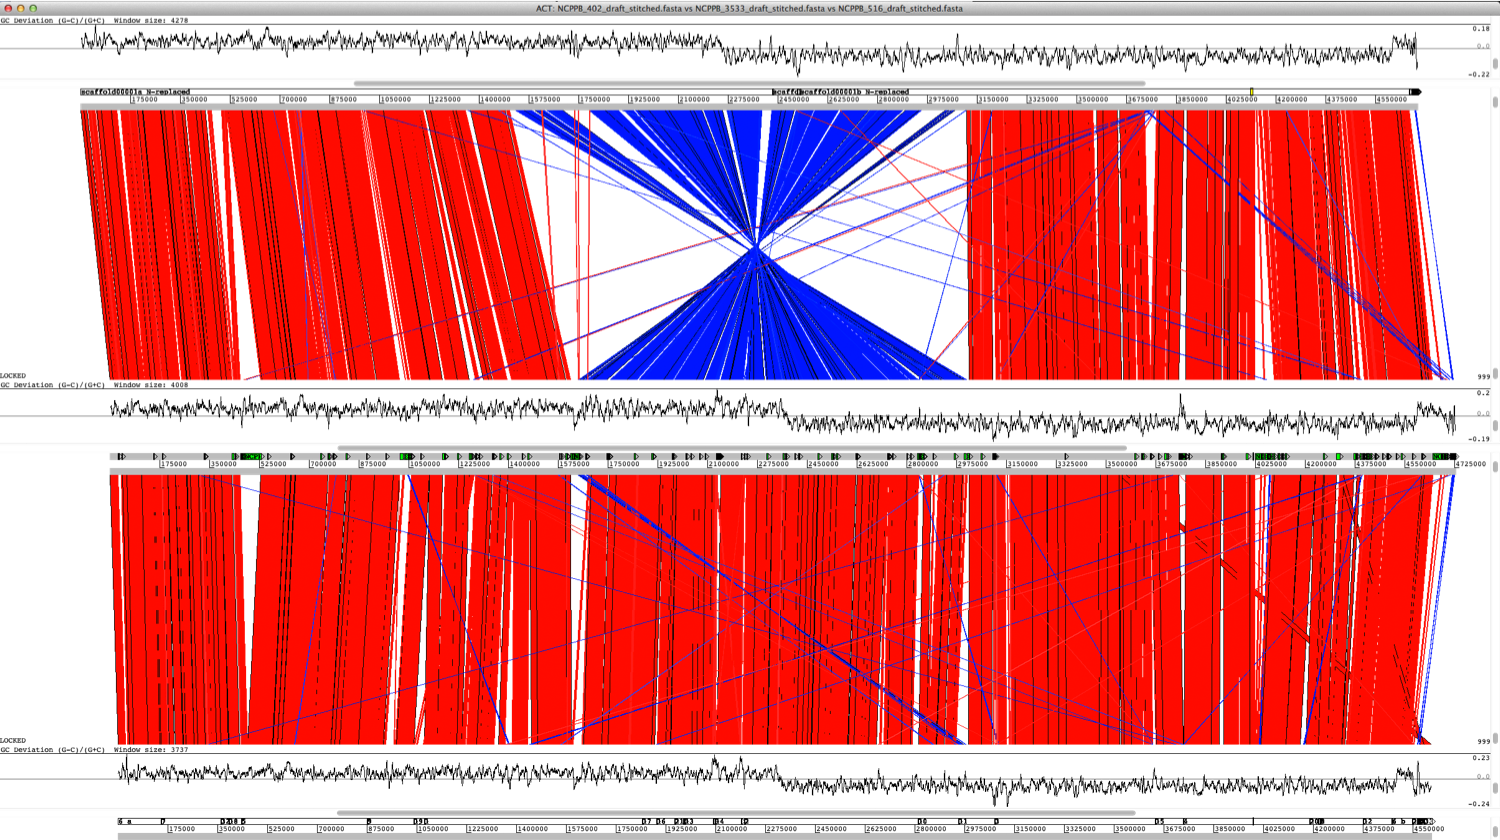
\includegraphics[width=\textwidth]{images/pairwise_genome_alignment}
  \end{center}  
\end{frame}

% SYNTENY AND COLLINEARITY
\begin{frame}
  \frametitle{Synteny and Collinearity}
  \textcolor{olive}{Genome rearrangements may occur post-species divergence} \\
  Sequence similarity, and order of similar regions, may be conserved
  \begin{center}
    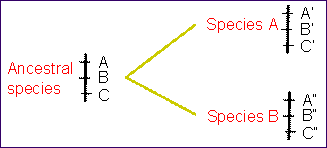
\includegraphics[width=0.5\textwidth]{images/collinear}    
    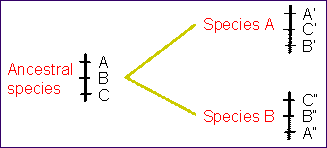
\includegraphics[width=0.5\textwidth]{images/synteny}
  \end{center}    
  \begin{itemize}
    \item \textcolor{hutton_blue}{\textit{collinear}} conserved elements lie in the same linear sequence
    \item \textcolor{hutton_purple}{\textit{syntenous} (or \textit{syntenic})} elements:
    \begin{itemize}
      \item (\textit{orig.}) lie on the same chromosome
      \item (\textit{mod.}) are collinear
    \end{itemize}
  \end{itemize}
  \textcolor{hutton_green}{Evolutionary constraint} (e.g. indicated by synteny) may indicate \textcolor{hutton_green}{functional constraint} (and help determine \textit{orthology})
\end{frame}

% VIBRIO MIMICUS
\begin{frame}
  \frametitle{\textit{Vibrio mimicus} 
  \footnote{\tiny{\href{http://dx.doi.org/10.1073/pnas.1013825107}{Hasan \textit{et al}. (2010) \textit{Proc. Natl. Acad. Sci. USA} \textbf{107}:21134-21139 doi:10.1073/pnas.1013825107}}}
  }
  \begin{alertblock}{Chromosomes}
    \begin{itemize}
      \item C-I: virulence genes.
      \item C-II: environmental adaptation
    \end{itemize}
  \end{alertblock}
  \textcolor{hutton_green}{C-II has undergone extensive rearrangement}; C-I has not.\\
  \begin{center}
    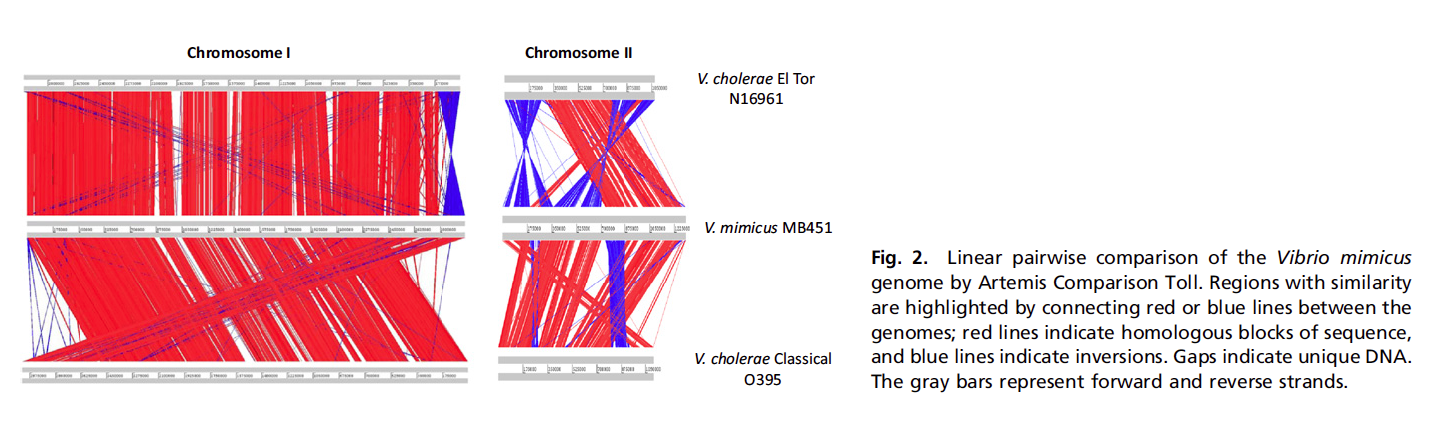
\includegraphics[width=1\textwidth]{images/v_mimicus}
  \end{center}    
  Suggests \textcolor{hutton_blue}{modularity of genome organisation, as a mechanism for adaptation} (HGT, two-speed genome).
\end{frame}

% SERRATIA SYMBIOTICA
\begin{frame}
  \frametitle{\textit{Serratia symbiotica} 
  \footnote{\tiny{\href{http://dx.doi.org/10.1093/gbe/evr002}{Burke and Moran (2011) \textit{Genome Biol. Evol.} \textbf{3}:195-208 doi:10.1093/gbe/evr002}}}
  }
  \textit{S. symbiotica} is a recently evolved symbiont of aphids\\
  \textcolor{hutton_green}{Massive genomic decay: consequence of adaptation}\\
  \begin{center}
    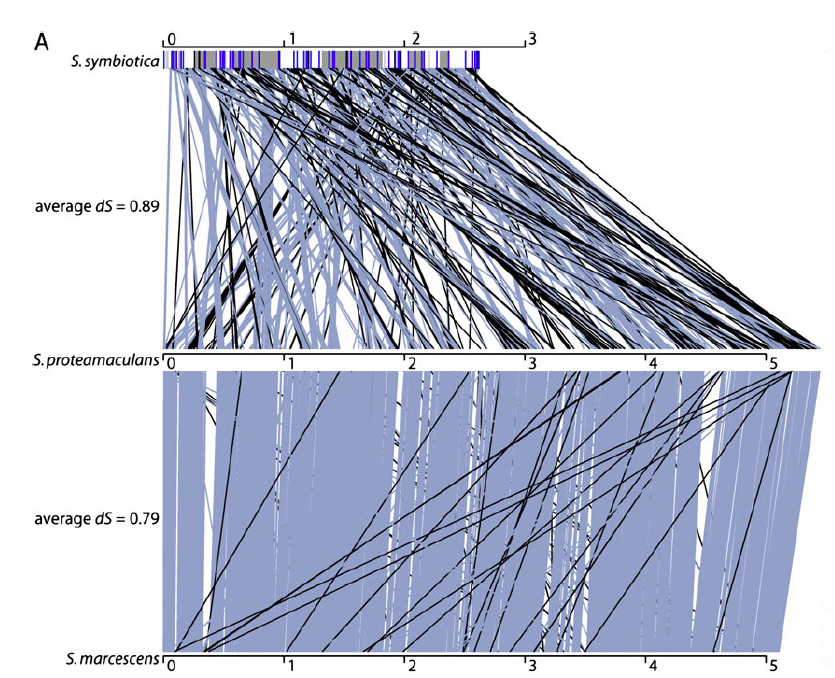
\includegraphics[width=0.75\textheight]{images/s_symbiotica}
  \end{center}    
\end{frame}


% WHOLE GENOME CLASSIFICATION
\begin{frame}
  \frametitle{Whole genome classification
  \footnote{\tiny{\href{http://dx.doi.org/10.1016/j.tim.2016.02.004}{Baltrus (2016) \textit{Trends Microbiol.} doi:10.1016/j.tim.2016.02.004}}}
    \footnote{\tiny{\href{http://dx.doi.org/10.1039/c5ay02550h}{Pritchard \textit{et al}. (2016) \textit{Anal. Methods} doi:10.1039/c5ay02550h}}}
  }
      \begin{itemize}  
        \item \textcolor{hutton_green}{Widespread confusion about strain classification and nomenclature}
          \begin{itemize}
            \item Taxonomies contradicted by bioinformatic classification
            \item Databases populated by non-taxonomists
          \end{itemize}
        \item \textcolor{hutton_blue}{Philosophy and practice of taxonomy are in conflict}
        \item \textcolor{hutton_purple}{Classification can be independent of existing nomenclature}
          \begin{itemize}
            \item The route from genotype to phenotype is complicated
            \item Time to abandon traditional microbial species concepts?
          \end{itemize}
          \item \textcolor{red}{An unambiguous sequence-based classification scheme is possible}
        \end{itemize}  
\end{frame}


% DNA-DNA HYBRIDISATION
\begin{frame}
  \frametitle{DNA-DNA hybridisation\footnote{\tiny{\href{http://dx.doi.org/10.1016/S0168-6445(00)00040-1}{Morello-Mora and Amann (2001) \textit{FEMS Micro. Rev.} doi:10.1016/S0168-6445(00)00040-1}}}}
  \begin{columns}[T]
    \begin{column}{5cm}
      \begin{itemize}
        \item ``Gold Standard'' for prokaryotic taxonomy, since 1960s. \textcolor{hutton_green}{``70\% identity $\approx$ same species.''}
        \item Denature DNA from two organisms.
        \item Allow to anneal. \textcolor{hutton_blue}{Reassociation $\approx$ similarity}, measured as $\Delta T$  of denaturation curves.
      \end{itemize}
    \end{column}
    \begin{column}{5cm}
      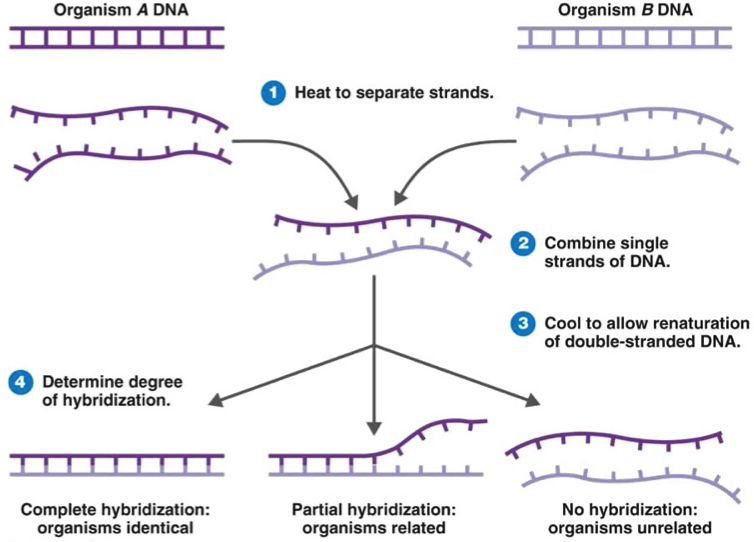
\includegraphics[width=1\textwidth]{images/dna-dna_hyb}
    \end{column}
  \end{columns}
\vspace{0.25cm}
\textcolor{hutton_purple}{Proxy for sequence similarity - replace with genome analysis\footnote{\tiny{\href{http://dx.doi.org/10.1186/1471-2180-12-302}{Chan \textit{et al} (2012) \textit{BMC Microbiol.} doi:10.1186/1471-2180-12-302}}}}?
\end{frame}

% ANIm
\begin{frame}
  \frametitle{Average Nucleotide Identity (ANIm)\footnote{\tiny{\href{http://dx.doi.org/10.1073/pnas.0906412106}{Richter and Rossello-Mora (2009) \textit{Proc. Natl. Acad. Sci. USA} doi:10.1073/pnas.0906412106}}}}
  \begin{columns}[T]
    \begin{column}{3cm}
      1. Align genomes (MUMmer)\\
      2. \textcolor{hutton_green}{\textbf{ANIm}: Mean \% identity of all matches} \\[0.25cm]
      \begin{itemize}
        \item DDH:ANIm linear
        \item \textcolor{hutton_blue}{70\%ID $\approx$ 95\%ANIb}
      \end{itemize}
    \end{column}
    \begin{column}{7cm}
      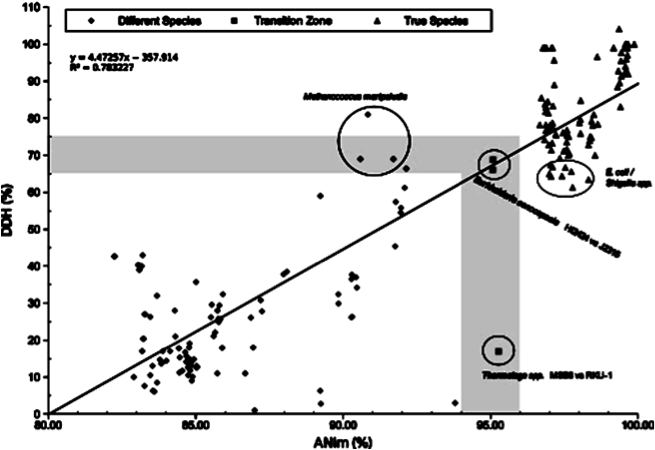
\includegraphics[width=1\textwidth]{images/ddh_anim}
    \end{column}
  \end{columns}
\end{frame}

% ANIm in practice
\begin{frame}
  \frametitle{55 Pectobacterium spp. ANIm
  \footnote{\tiny{\href{http://dx.doi.org/10.1039/c5ay02550h}{Pritchard \textit{et al}. (2016) \textit{Anal. Methods} doi:10.1039/c5ay02550h}}}
  }
  \begin{columns}[T]
    \begin{column}{3cm}
      \begin{itemize}
        \item Ten species-level groups (four novel)
        \item \small{\textit{P. carotovorum} split: several species}
        \item \small{\textit{P. wasabiae} split: two species}
      \end{itemize}
    \end{column}
    \begin{column}{7cm}
      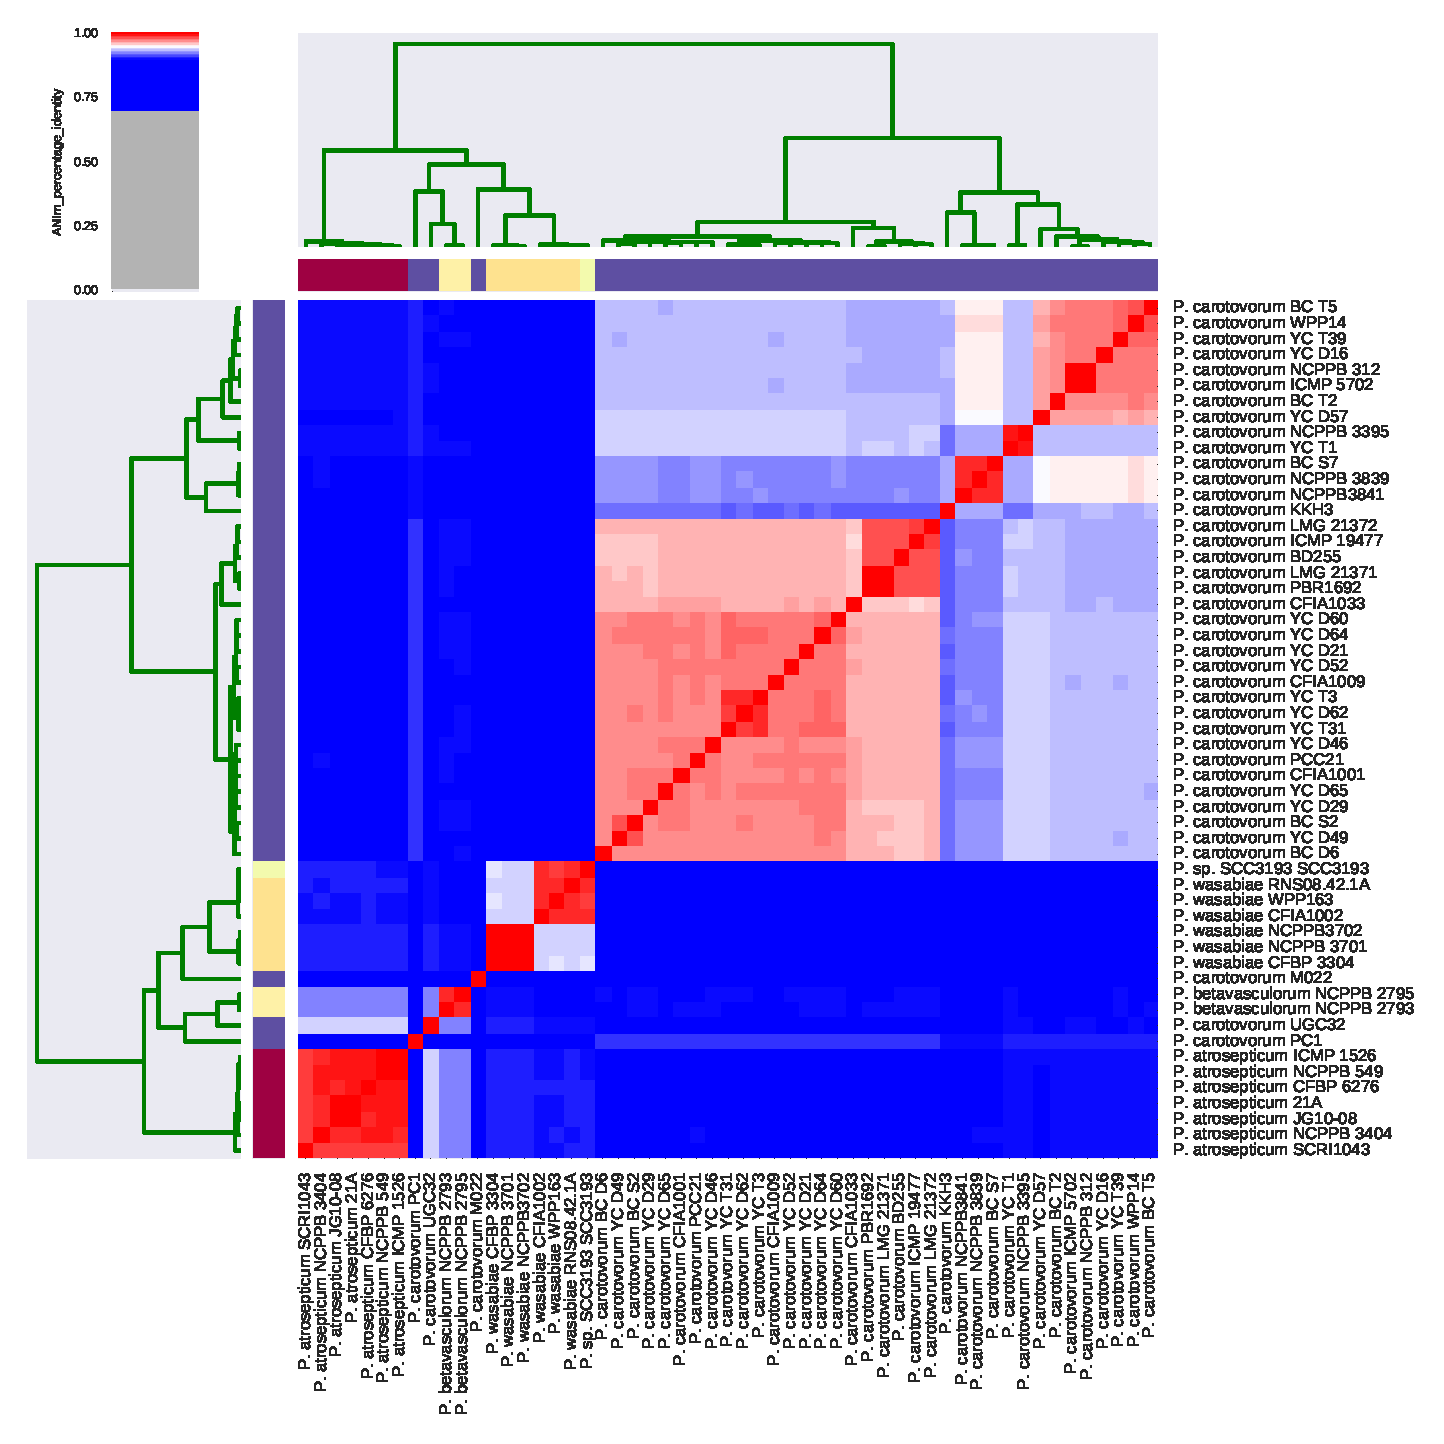
\includegraphics[width=1\textwidth]{images/Pectobacterium_ANIm_percentage_identity}
    \end{column}
  \end{columns}
\end{frame}

% ANIm in practice
\begin{frame}
  \frametitle{55 Pectobacterium spp. ANIm\footnote{\tiny{\href{http://dx.doi.org/10.1039/c5ay02550h}{Pritchard \textit{et al}. (2016) \textit{Anal. Methods} doi:10.1039/c5ay02550h}}}}
  \begin{columns}[T]
    \begin{column}{3cm}
      \begin{itemize}
        \item All isolates align over $>$50\% of whole genome
      \end{itemize}
    \end{column}
    \begin{column}{7cm}
      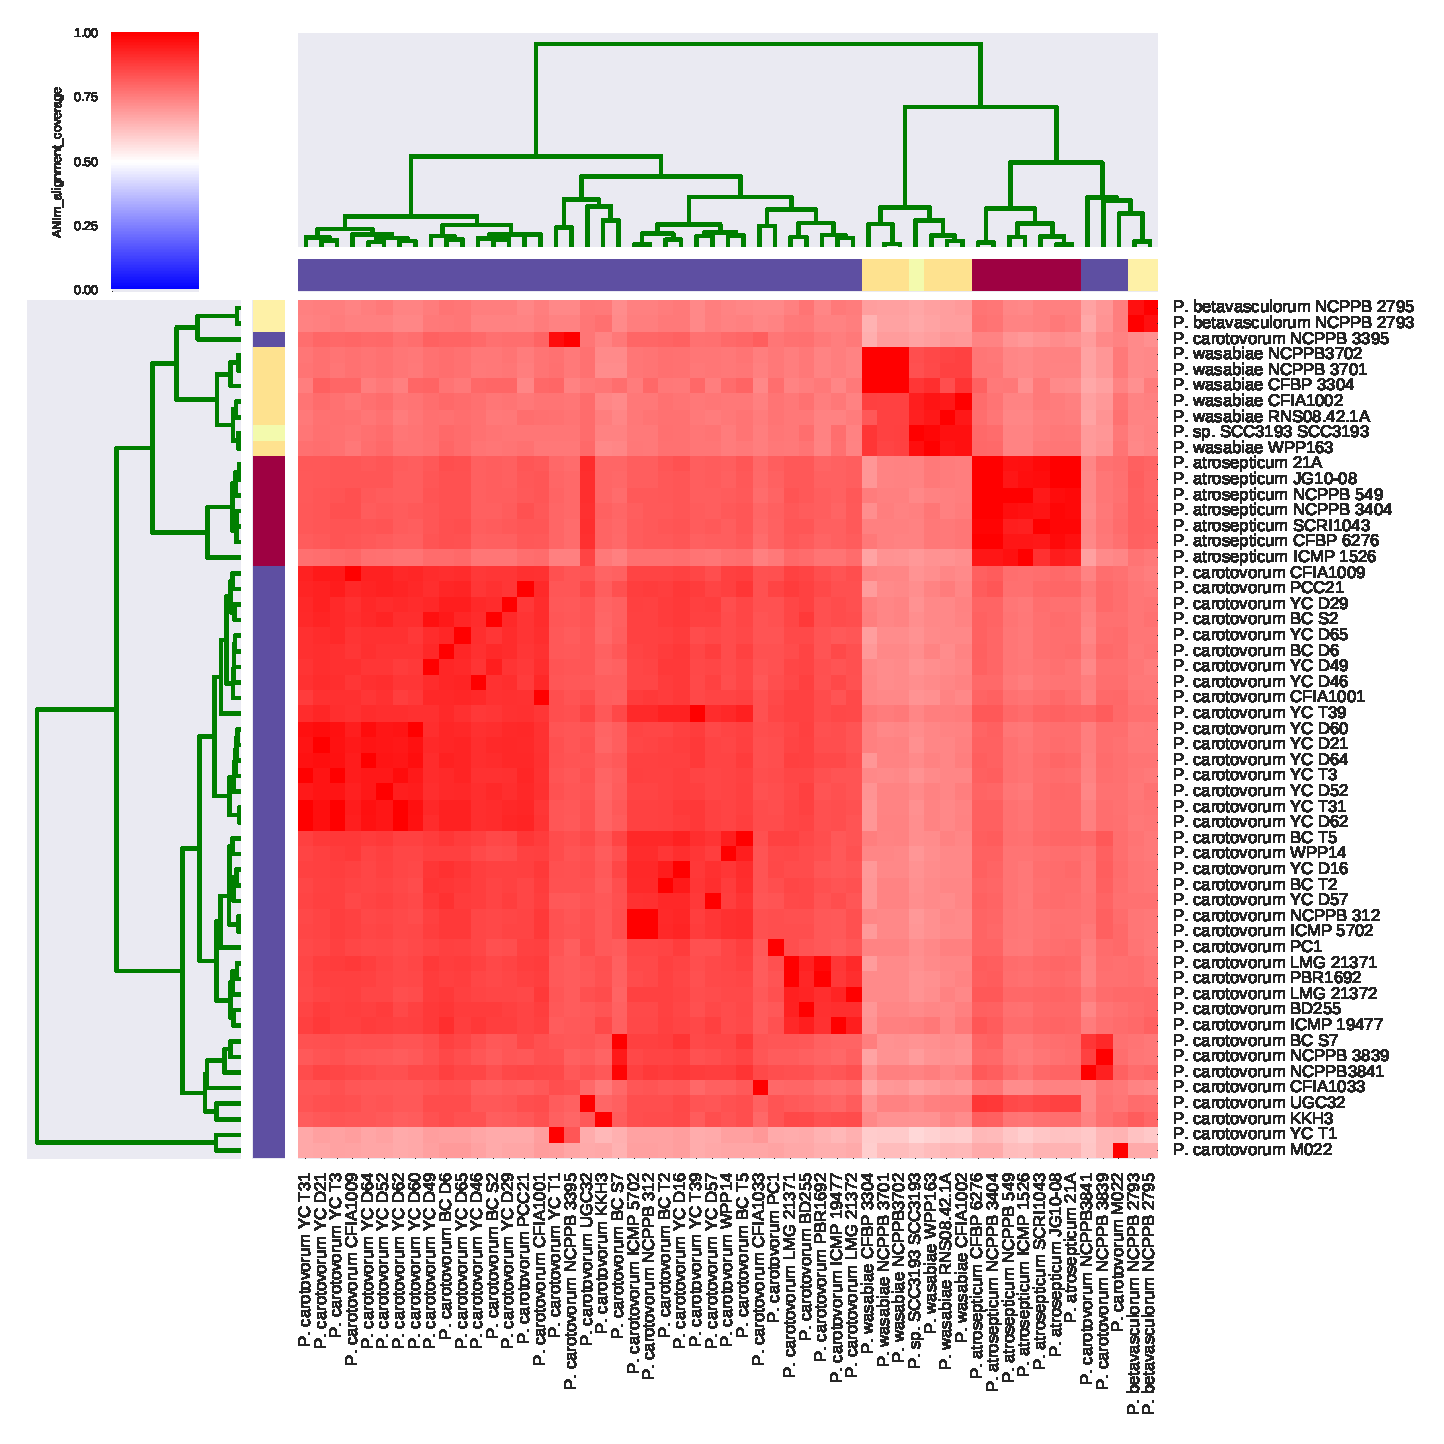
\includegraphics[width=1\textwidth]{images/Pecto_ANIm_alignment_coverage}
    \end{column}
  \end{columns}
\end{frame}

% ANI
\begin{frame}
  \frametitle{ANI}
  \begin{alertblock}{Advantages}
    \begin{itemize}
      \item Average identity of all `homologous' regions
      \item Approximates limiting case of MLST/MLSA/multigene comparisons
      \item Adaptable to variable thresholding (LINS) classifications
    \end{itemize}    
  \end{alertblock}
  \begin{block}{Criticisms}
    \begin{itemize}
      \item Thresholds `arbitrary', based on homologous regions only
      \item Taxonomic classification, not phylogenetic reconstruction
      \item No functional (or gene-based) interpretation; still need pangenome classification and analysis
    \end{itemize}
  \end{block}
\end{frame}

% EXERCISE
\begin{frame}
  \frametitle{EXERCISE}
  \begin{alertblock}{\url{exercises/01-whole_genome_comparisons.ipynb}}
    \begin{itemize}
      \item Pairwise comparison of \textit{Pseudomonas} genomes
      \item ANIm classification of \textit{Pseudomonas} isolates
    \end{itemize}
  \end{alertblock}
  \begin{itemize}
    \item \textcolor{hutton_purple}{\href{http://mybinder.org/repo/widdowquinn/Teaching-EMBL-Plant-Path-Genomics}{MyBinder link}}
  \end{itemize}
\end{frame}

% CHROMOSOME PAINTING
\begin{frame}
  \frametitle{Chromosome painting
  \footnote{\tiny{\href{http://dx.doi.org/10.1093/molbev/mst055}{Yahara \textit{et al}. (2013) \textit{Mol. Biol. Evol.} \textbf{30}:1454-1464 doi:10.1093/molbev/mst055}}}
  }
  \begin{itemize}
    \item ``Chromosome painting'' (\textcolor{hutton_purple}{\href{http://www.paintmychromosomes.com/}{FINESTRUCTURE}}) infers recombination-derived `chunks'\\
    \item Genome's haplotype constructed in terms of recombination events from a `donor' to a `recipient' genome\\
  \end{itemize}
  \begin{center}
    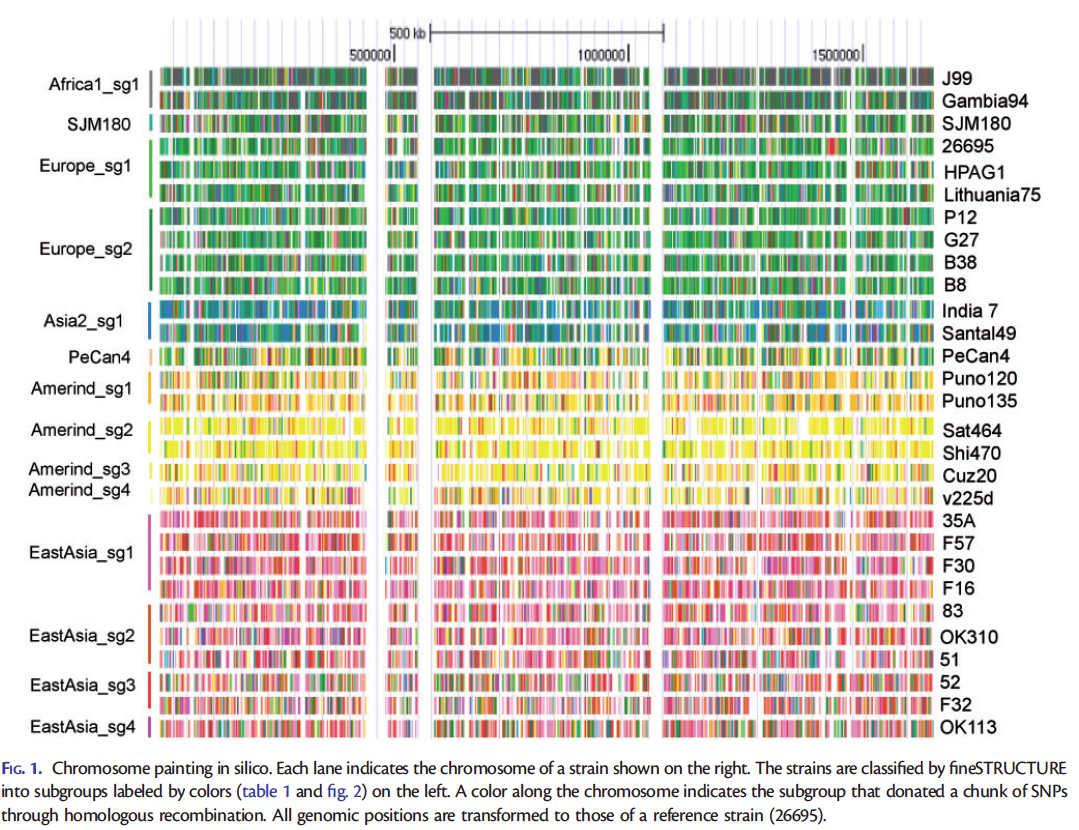
\includegraphics[width=0.6\textwidth]{images/chromosome_painting}
  \end{center}     
\end{frame}

% DNA-DNA hybridisation
\begin{frame}
  \frametitle{Chromosome painting
  \footnote{\tiny{\href{http://dx.doi.org/10.1093/molbev/mst055}{Yahara \textit{et al}. (2013) \textit{Mol. Biol. Evol.} \textbf{30}:1454-1464 doi:10.1093/molbev/mst055}}}
  }
  \begin{itemize}
    \item Recombination events summarised in a \textit{coancestry matrix}.\\
    \item \textit{H. pylori}: most within geographical bounds, but asymmetrical donation from Amerind/East Asian to European isolates.
  \end{itemize}
  \begin{center}
    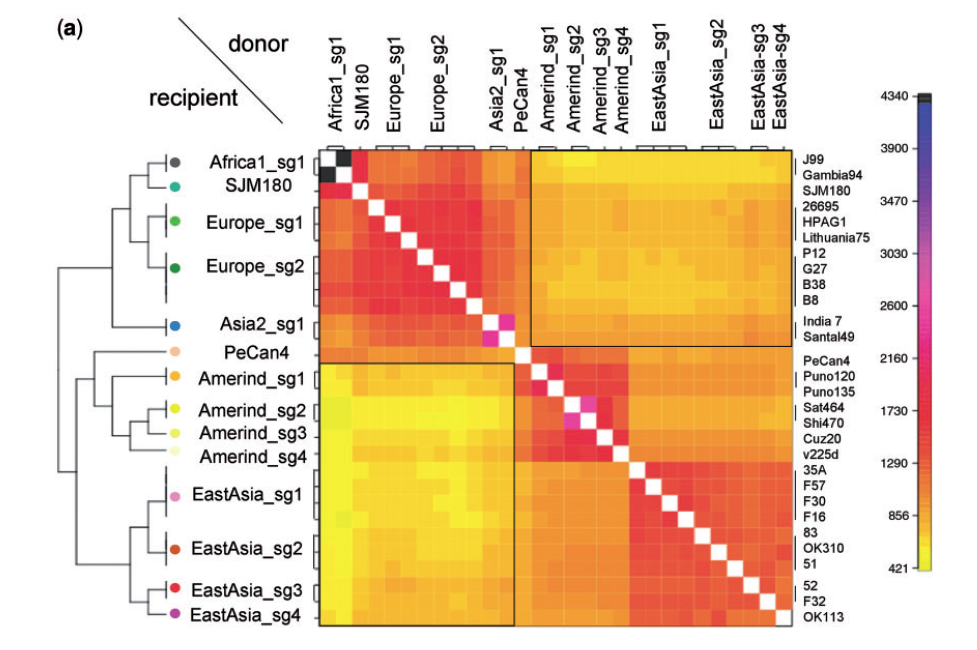
\includegraphics[width=0.75\textwidth]{images/coancestry}
  \end{center}     
\end{frame}